% !TEX TS-program = lualatex
% !TEX encoding = UTF-8

\documentclass[12pt]{article} % use larger type; default would be 10pt

\usepackage{geometry} % See geometry.pdf to learn the layout options. There are lots.
\usepackage{graphicx} % support the \includegraphics command and options
\geometry{a4paper} % or letterpaper (US) or a5paper or....
\usepackage[allowdeprecated=false]{gregoriotex} % for gregorio score inclusion
\usepackage{fullpage} % to reduce the margins
\usepackage[oldstyle]{libertine}
\usepackage{lettrine}
\usepackage{fancyhdr}
\usepackage{titlesec}
\pagestyle{fancy}
\lhead{}
\chead{\color{benred8}\textsc{Quicumque vult: the Athanasian Creed}}
\rhead{}
\lfoot{}
\cfoot{\textcolor{benblue1}{\thepage}}
\rfoot{}
\renewcommand{\headrulewidth}{0pt}
\setlength{\headsep}{25pt}
%redefine 'plain' page style to have blue page numbers too
\fancypagestyle{plain}{
    \chead{}
    \cfoot{\textcolor{benblue1}{\thepage}}

}

\setlength{\parindent}{-0.25in}
\usepackage[normalem]{ulem}
\setlength{\ULdepth}{2pt}

\definecolor{benred8}{HTML}{E82C00}
\definecolor{benblue1}{HTML}{2B22C7}
\definecolor{benyellow1}{HTML}{FFD435}
\definecolor{benyellow2}{HTML}{7C6F3B}

% FORMAT SECTIONS - use titlesec package
\titleformat{\section}{\centering\scshape\Huge\color{benred8}}{}{1em}{}
\titlespacing*{\section}{0pt}{0pt}{0pt}

\usepackage{amsmath}
\newcommand{\madlib}[1]{\uline{\hspace{3em}}$_{\color{benred8}\text{#1}}$}

%%%%%%%%%%%%%%%%%%%%%%%%%%%%
% HERE BEGINS THE DOCUMENT %
%%%%%%%%%%%%%%%%%%%%%%%%%%%%

\begin{document}

\thispagestyle{plain}

\section*{Quicumque vult: the Athanasian Creed}

\vspace{1mm}

\lettrine{W}{hosoever} wishes to be~\madlib{a} must, above all, keep the~\madlib{b} faith. For unless a person keeps this faith whole and entire, he will undoubtedly be~\madlib{c} forever. This is what the~\madlib{b} faith teaches: we worship one God in the Trinity and the Trinity in unity. Neither confounding the Persons, nor dividing the substance. For there is one Person of the Father, another of the Son, another of the Holy Spirit. 

\lettrine{B}{ut} the Father and the Son and the Holy Spirit have one divinity, equal glory, and co\madlib{g} majesty. What the Father is, the Son is, and the Holy Spirit is. 

\lettrine{T}{he} Father is uncreated, the Son is uncreated, and the Holy Spirit is uncreated. The Father is boundless, the Son is boundless, and the Holy Spirit is boundless. The Father is~\madlib{g}, the Son is~\madlib{g}, and the Holy Spirit is~\madlib{g}. 

\lettrine{N}{evertheless}, there are not three~\madlib{g} beings, but one~\madlib{g} being. So there are not three uncreated beings, nor three boundless beings, but one uncreated being and one boundless being. Likewise, the Father is omnipotent, the Son is omnipotent, the Holy Spirit is omnipotent. 

\lettrine{Y}{et} there are not three omnipotent beings, but one omnipotent being. Thus the Father is God, the Son is God, and the Holy Spirit is God. 

\lettrine{H}{owever}, there are not three gods, but one God. The Father is Lord, the Son is Lord, and the Holy Spirit is Lord. However, there are not three lords, but one Lord. For as we are obliged by~\madlib{e} truth to acknowledge every Person singly to be God and Lord, so too are we~\madlib{d} by the~\madlib{b} religion to say that there are three Gods or Lords. 

\lettrine{T}{he} Father was not made, nor created, nor~\madlib{f} by anyone. The Son is not made, nor created, but~\madlib{f} by the Father alone. The Holy Spirit is not made, nor created, nor~\madlib{f}, but proceeds from the Father and the Son. There is, then, one Father, not three Fathers; one Son, not three sons; one Holy Spirit, not three holy spirits. In this Trinity, there is nothing before or after, nothing greater or less. The entire three Persons are co\madlib{g} and coequal with one another. So that in all things, as is has been said above, the Unity is to be~\madlib{h} in Trinity and the Trinity in Unity. 

\lettrine{H}{e}, therefore, who wishes to be~\madlib{a}, must believe thus about the Trinity. It is also~\madlib{j} for~\madlib{g} salvation that he believes steadfastly in the incarnation of our Lord Jesus Christ. Thus the right faith is that we believe and confess that our Lord Jesus Christ, the Son of God, is both God and man. As God, He was~\madlib{f} of the substance of the Father before time; as man, He was born in time of the substance of His Mother. He is perfect God; and He is perfect man, with a~\madlib{i} soul and human flesh. He is equal to the Father in His divinity, but inferior to the Father in His humanity. Although He is God and man, He is not two, but one Christ. And He is one, not because His divinity was~\madlib{k} into flesh, but because His humanity was assumed unto God. He is one, not by a mingling of substances, but by unity of person. As a~\madlib{i} soul and flesh are one man: so God and man are one Christ. He died for our salvation, descended into Hell, and rose from the dead on the third day. He ascended into Heaven, sits at the right hand of God the Father almighty. From there He shall come to judge the living and the dead. At His coming, all men are to arise with their own bodies; and they are to give an account of their own deeds. Those who have done good deeds will go into~\madlib{g} life; those who have done evil will go into the~\madlib{g} fire. 

\lettrine{T}{his} is the~\madlib{b} faith. Everyone must believe it, firmly and steadfastly; otherwise He cannot be~\madlib{a}. Amen.

\newpage

\begin{Huge}
\begin{center}

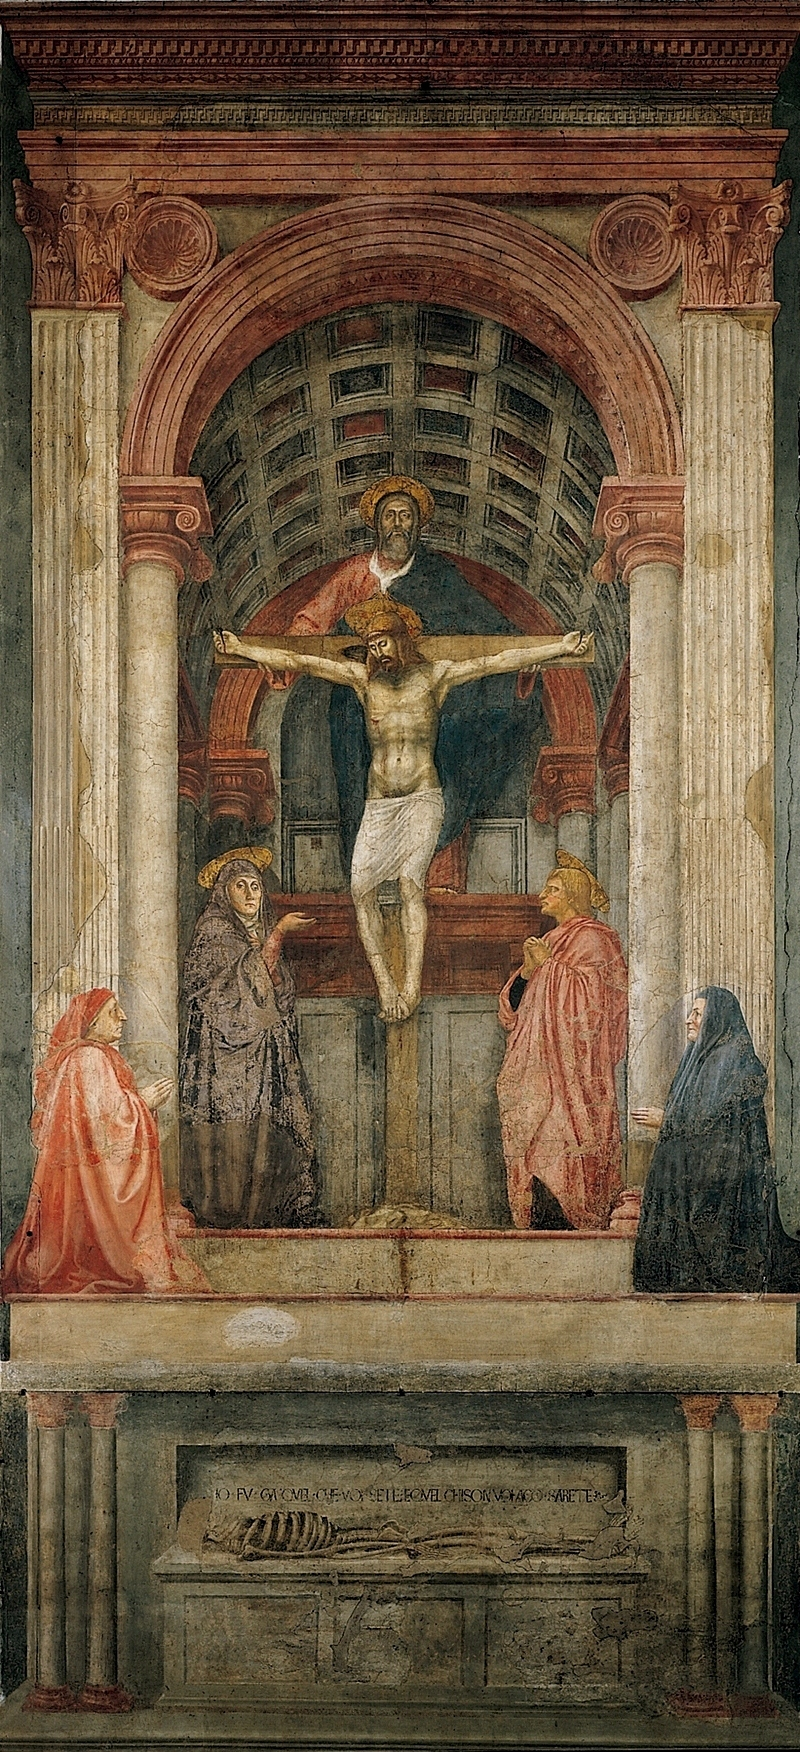
\includegraphics[height=4.25in]{Masaccio-Trinity.jpg}

\vspace{0.25in}

\begin{tabular}{ c c c }
 a & \hspace{10em} & Christian \\ 
 b &  & worshipped \\  
 c &  & necessary \\ 
 d &  & lost \\
 e &  & eternal \\
 f &  & Catholic \\
 g &  & changed \\
 h &  & rational \\
 i &  & forbidden \\
 j &  & saved \\
 k &  & begotten
\end{tabular}
\end{center}
\end{Huge}

\end{document}
